\documentclass[letterpaper,12pt]{extarticle}%Preambulo
\usepackage[utf8]{inputenc}%Preambulo
\usepackage[spanish,mexico]{babel}%Preambulo
\usepackage{ae}
\usepackage{amsmath,amssymb,amsfonts,latexsym,cancel}%Preambulo
\usepackage{hyperref}%Preambulo
\usepackage[pdftex]{graphicx}%Preambulo
\usepackage{wrapfig}%Preambulo
\usepackage[rflt]{floatflt}%Preambulo
\usepackage{fancyhdr}%%Pre?mbulo
\usepackage{mathptmx}%%Pre?mbulo
\usepackage{float}%%Pre?mbulo
\usepackage{longtable,multirow,booktabs}%%Pre?mbulo
%\usepackage{cite}
\usepackage{wrapfig}%%Pre?mbulo
\usepackage[rflt]{floatflt}%%Pre?mbulo
\usepackage{natbib} %%Pre?mbulo
\usepackage{multicol}%%Pre?mbulo
\usepackage{caption}%%Pre?mbulo
\usepackage{geometry}
\usepackage{wrapfig}
\usepackage{adjustbox}
\usepackage{amsmath}
\usepackage{parskip}
\usepackage{tikz}
\usepackage{lipsum}
\usepackage{xcolor}
\usepackage[T1]{fontenc}

\captionsetup{
       font=small,
       labelfont=bf,
       tableposition=top,
       hypcap=false
    }

\DeclareGraphicsExtensions{.pdf, .png, .jpg, .PNG, .JPG}%Cuando ponemos im?genes ya no es necesario poner la extensi?n

%%%FORMATO DE LA P?GINA%%%
\textheight = 21cm %Medidas de la  p?gina
\textwidth = 18cm  %Medidas de la p?gina
\topmargin = -1cm  %Medidas de la p?gina    
\oddsidemargin = -1cm %Medidas de la p?gina
\pagestyle{fancy} %Dise?o de la p?gina
\lhead{Universidad de la Sierra Sur}%%LeftHead
\chead{
\includegraphics[width=1cm, height=1cm]{imag//logL}}%%CenterHead
%\lfoot{USM}
\rhead{Licenciatura en Informática}%%RightHead
%\lfoot{Gonz?lez Chico Juan Daniel} %Pie de pagina izquierdo

\setlength{\columnsep}{7mm}%Comandos para el formato de la p?gina
%\setlength{\parindent}{4em}%Sangr?a al comenzar un nuevo p?rrafo
\setlength{\parindent}{0.5in}
%\setlength{\parindent}{4em}%Sangr?a al comenzar un nuevo p?rrafo
\setlength{\parskip}{1em}%distancia entre p?rrafos
\renewcommand{\baselinestretch}{1.0}% Espacio entre l?nea y l?nea
\setlength{\headheight}{33pt}

\hypersetup{
	colorlinks = true,
	linkcolor = black,
	urlcolor = cyan
}
\urlstyle{same}

\begin{document}

    \begin{titlepage}
		% Mine page for add image at scale with footer image in 
		\begin{figure}[ht]
		   \minipage{0.76\textwidth}
				
\includegraphics[width=4cm]{imag//logColor.jpg}
				\label{escudoFI}
		   \endminipage
		   \minipage{0.32\textwidth}

				
\includegraphics[height = 4.5cm ,width=4cm]{imag//logBN.jpg} 
				\label{EscuoUNAM}
			\endminipage
				%%\vspace{-1cm}
		\end{figure}
		
		\vspace{0.5cm}
		
		\begin{center}
			\LARGE UNIVERSIDAD DE LA SIERRA SUR \\
			\vspace{0.3cm}
			\LARGE Instituto de Informática
			
			\vspace{.7cm} {\LARGE  \textbf{Torres de Hanoi} \\}

			% Incrementamos el interlineado:
			

			% Restauramos el interlineado:
			\vspace{.5cm}
			\begin{center}

				\LARGE{ \textbf{Alumnos:}}\\%% \textbf son negritas
        		\LARGE{Cruz Ortega Elio Justino}\\
				\LARGE{Galicia Cordova Elietzer Jared}\\%% \it es letra it?lica
				\LARGE{Gómez Hernández Yael Alberto}\\
				\LARGE{Marquez Espina José Angel}\\
				\LARGE{Zavaleta Cruz Jonathan Alexis}\\
				\vspace{0.5cm}
				\textbf{Profesor:}  Dr. Viztor Alberto Gómez Hernández \\
				\vspace{0.5cm}
				\textbf{Grupo:}  306
				
			\end{center}
			
			\vspace{1cm} \today
		\end{center}
	\end{titlepage}

    \newpage
    \tableofcontents
    \newpage
    
    \begin{center}
    {\it Grupo 306}\\[3mm]
    {\it Torres de Hanoi}\\[3mm]
    \end{center}
    

		% Inicio del documento

	% Section for links in doct e index
	\begin{multicols}{2}
    \section{Introducción}
		El juego de las torres de Hanoi, o también es conocido, de las torres de Brahma
		o el problema del fin del mundo, es un juego de normas sencillas, el proposito 
		principal del juego es encontrar una solución óptima y a partir de ella realizar 
		diversos conteos combinatorios.
		
		% % Coloca imagen y la centra en el espacio asignado
		% \begin{figure}[H]
		% \begin{center}
		% 
\includegraphics[width=4cm]{imag//logBN.jpg}
		% \caption{foto de escudo}
		% \label{figuraBN}
		% \end{center}
		% %%\vspace{-1cm}
 		% \end{figure}

		% ver la figura \ref*{figuraBN}
        
    \section{Descripción del juego}
		Este juego en su forma más básica está formada por 3 pilares verticales,
		una de ellas es denominada "origen", se apila una torre de n discos ordenado
		de mayor a menor tamaño, siendo el disco de mayor tamaño la base.
		El objetivo de este juego es mover la torre del pilar origen al pilar destino
		con el menor número de movimientos posible.
		Para conseguirlo se deben seguir las siguientes 2 simples reglas:
    \begin{enumerate}
	
		\item Solo se moverá un disco a la vez.

		\item No se podra colocar un disco de mayor tamaño sobre otro de menor tamanño.
	
	\end{enumerate} 
		% Coloca imagen y la centra en el espacio asignado
		% \begin{figure}[H]
		% \begin{center}
		% 
\includegraphics[width=4cm]{imag//logColor.jpg}
		% \caption{foto de escudo}
		% Convertidor
		% \label{figura}
		% \end{center}
		% %%\vspace{-1cm}
 		% \end{figure}

		% ver figura \ref{figura} se observa....
    
		
	\section{Desarrollo}
	\subsection{Estrategia}
		Lo importante antes de comenzar a contar el número de movimientos necesarios
		para resolver el juego, y otros problemas combinatorios asociados, es tener
		una solución del juego y poder garantizar que la solución es optima.
	\subsection{Diseño y creación de algoritmos}
		Creamos una estructura para cambiar el tamaño de la imagen.
	

		% Coloca imagen de diseño de imagen
		\begin{figure}[H]
		\begin{center}
		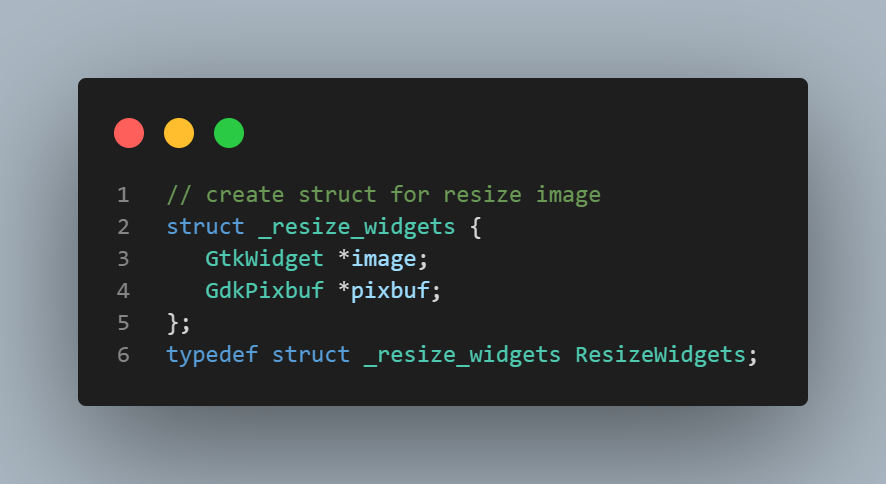
\includegraphics[width=7cm]{imag//img1.png}
		\caption{}
		% Convertidor
		\label{ProgramDesign}
		\end{center}
		%%\vspace{-1cm}
 		\end{figure}
		
		Crea un botón, configura la imagen, agrega la máscara de eventos y conecta
		button press event y motion notify event señala las funciones apropiadas.

		% Coloca imagen de diseño de imagen
		\begin{figure}[H]
		\begin{center}
		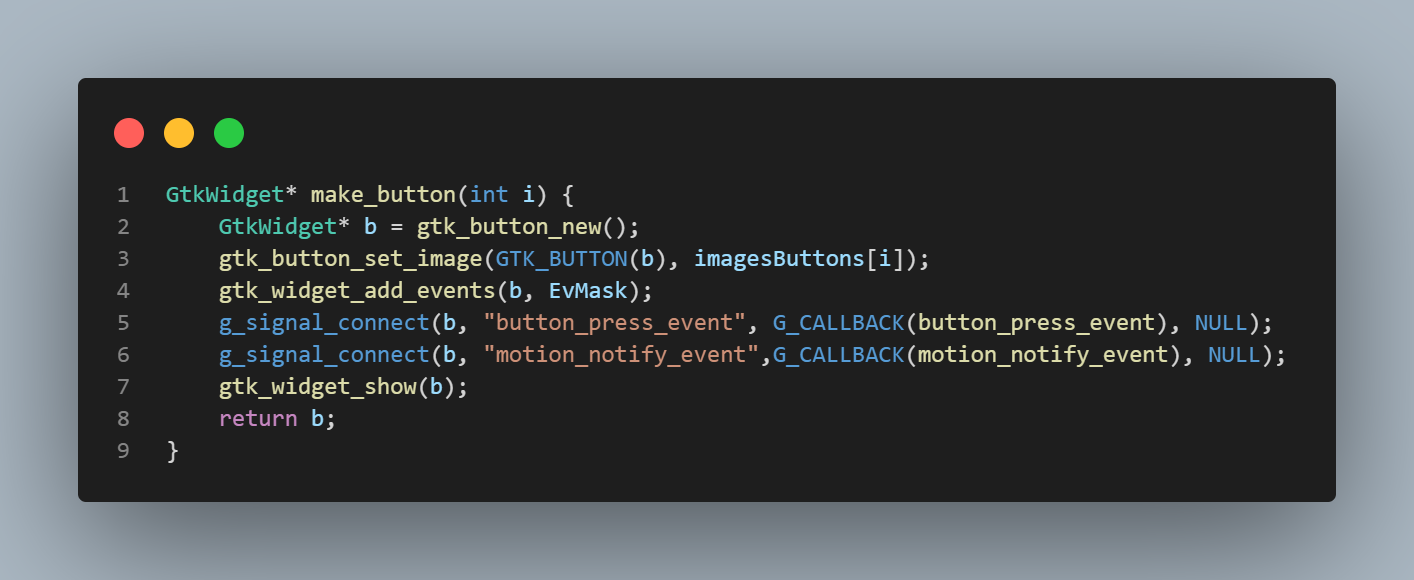
\includegraphics[width=7cm]{imag//img2.png}
		\caption{}
		% Convertidor
		\label{decToOct}
		\end{center}
		%\vspace{-1cm}
		\end{figure}

		Crea una pila con la cantidad de discos que el usuario ha elegido, y luego
		crea un botón para cada disco, y luego muestra la torre.

		% Coloca imagen de diseño de imagen
		\begin{figure}[H]
			\begin{center}
			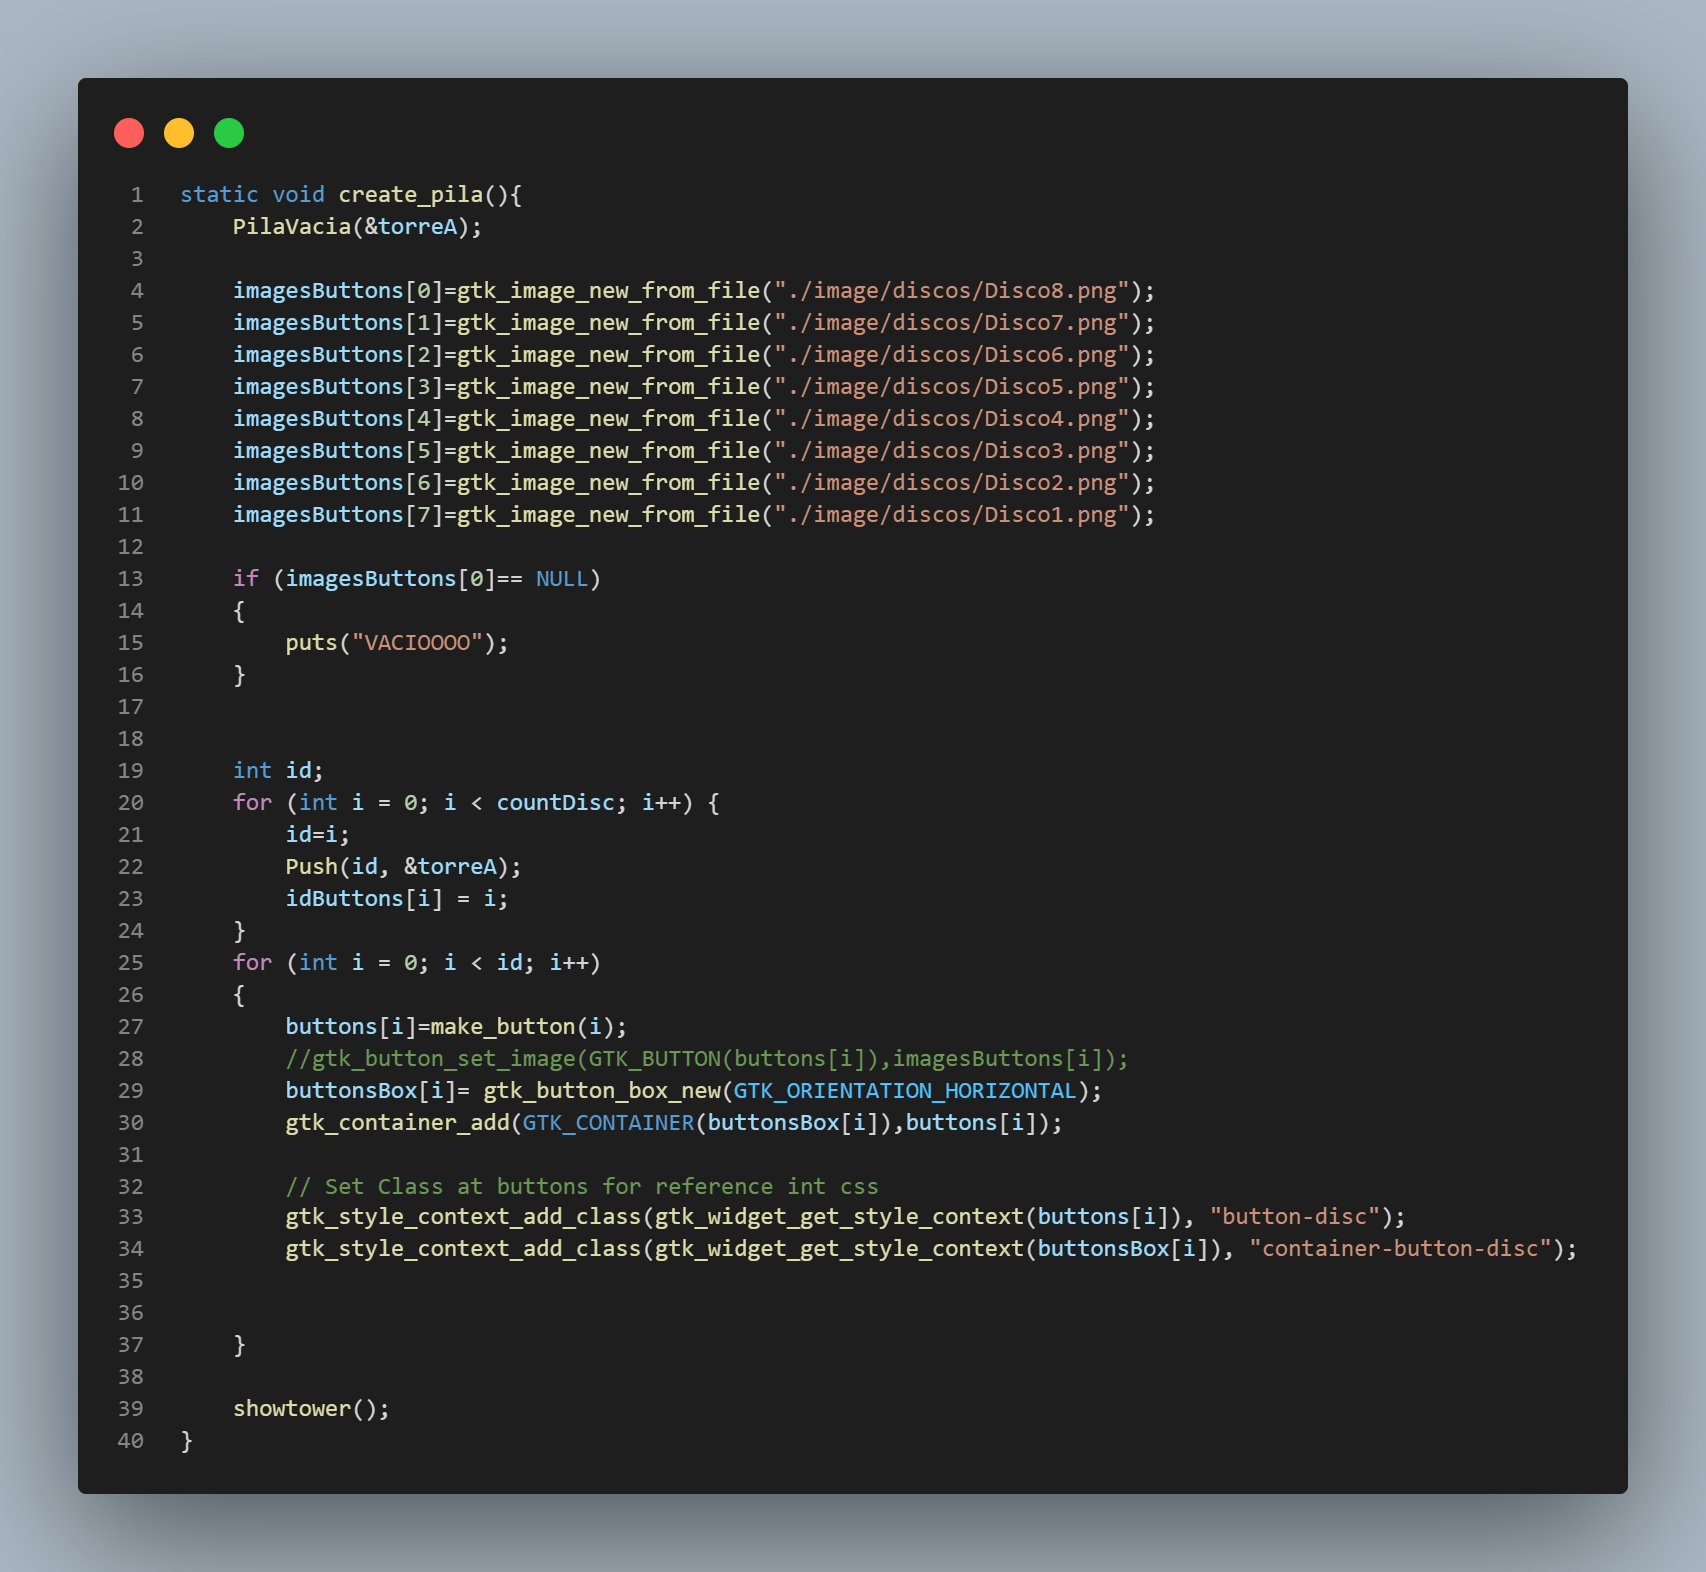
\includegraphics[width=9cm]{imag//img4.png}
			\caption{}
			% Convertidor
			\label{algDecToRest}
			\end{center}
			%\vspace{-1cm}
			\end{figure}

			Obtiene el número de discos del cuadro combinado y establece
			la variable global countDisc en ese número
			% Coloca imagen de diseño de imagen
			\begin{figure}[H]
			\begin{center}
			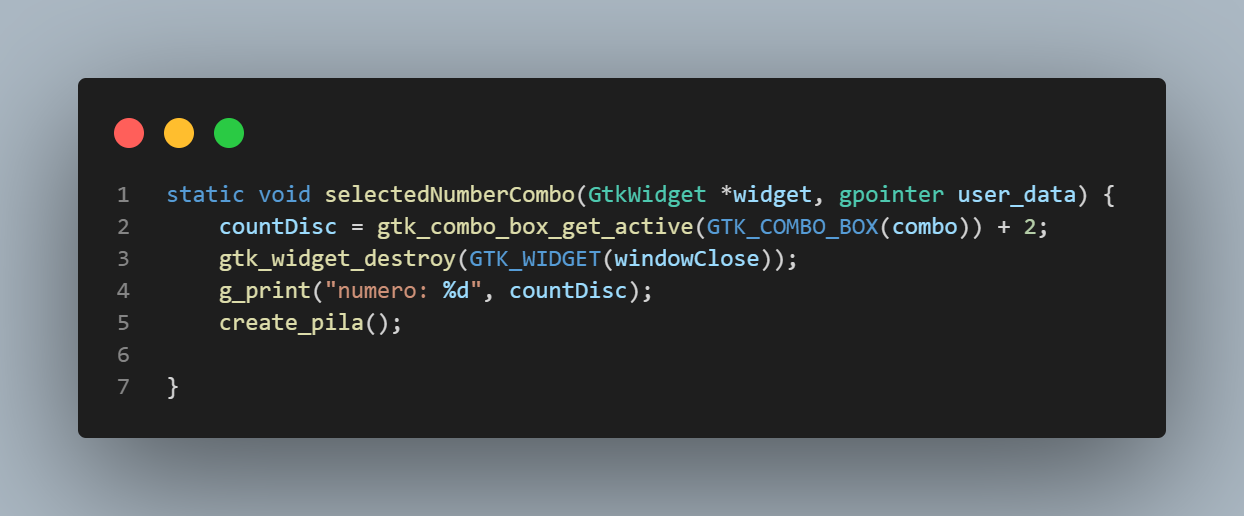
\includegraphics[width=9cm]{imag//img7.png}
			\caption{}
			% Convertidor
			\label{algBinToDec}
			\end{center}
			%\vspace{-1cm}
			\end{figure}

			Imprime la hora en formato 00:00:00, y lo hace cada segundo.
			% Coloca alg de BCD a decimal
			\begin{figure}[H]
			\begin{center}
			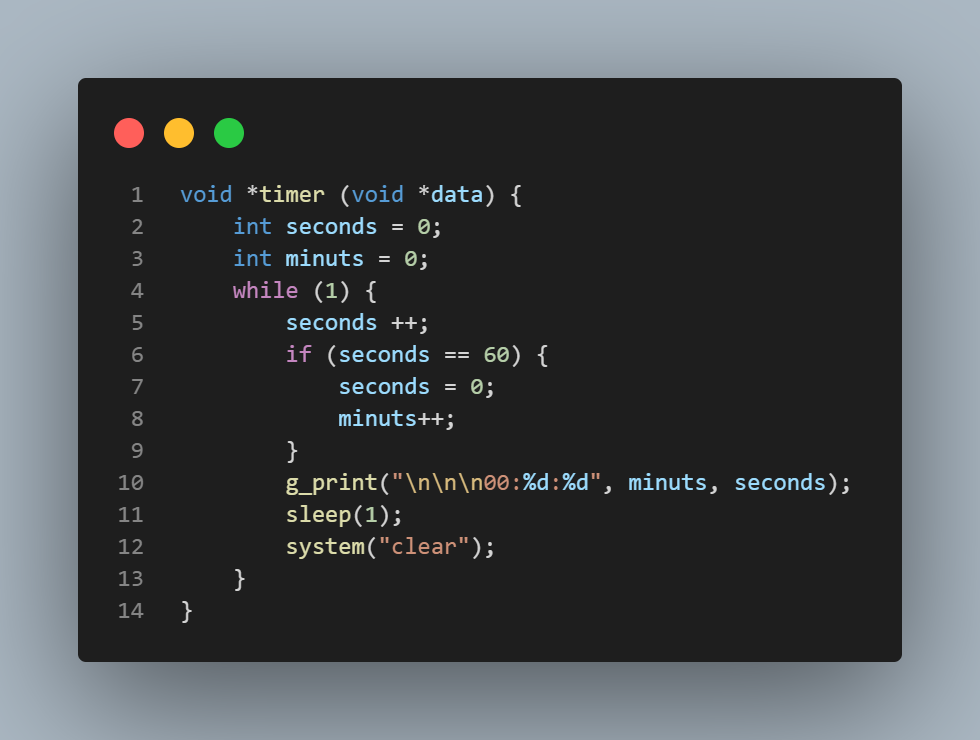
\includegraphics[width=10cm]{imag//img8.png}
			\caption{}
			% Convertidor
			\label{algBcdToDec}
			\end{center}
			%\vspace{-1cm}
			\end{figure}
    
    	
    \section{Resultados}
		 De manera general conseguimos hacer un programa que no solo funcionara si no que
		 también tubiera el interfaz lo más parecido a un videojuego, de igual forma 
		 realizamos funciones que pueden dar un toque extra así como un contador e incluso
		 una lista de que nos puede mostrar el puntaje y un top de los jugadores que han 
		 conseguido terminar el juego con los minimos movimientos posibles y el tiempo en 
		 que fue completado el juego.

		

	    \end{multicols}
	    \section{Conclusiones}
		El programa fue completado con exito, si que es verdad que hubieron complicaciones como por ejemplo la creación del contador, al principio fue una idea que no teniamos contemplada por completo, por que el meter un contador implicaba crear una tabla que mostrará un ranking, en el cual mostraría una columna que mostrará el nombre del jugador, la cantidad de movimientos que realizó y el tiempo en que tardó en terminar el juego.
		
		Código fuente: \url{https://github.com/UnsisWorks/hannoi-With-Gtk.git}
    
	\newpage
	
	% \section{Anexo de ecuaciones}
	
	% En caso des ser necesario se deben agregar ecuaciones que se hayan empleado

	% %Agrega todo lo ingresado tal cual
	% \begin{verbatim}
	% 	!"##$$%&%&/()
	% \end{verbatim}

	\cfoot{\LaTeX}
\end{document}